\h{Disclaimer}

\vspace{1cm}

\begin{figure}[h]
    \centering
    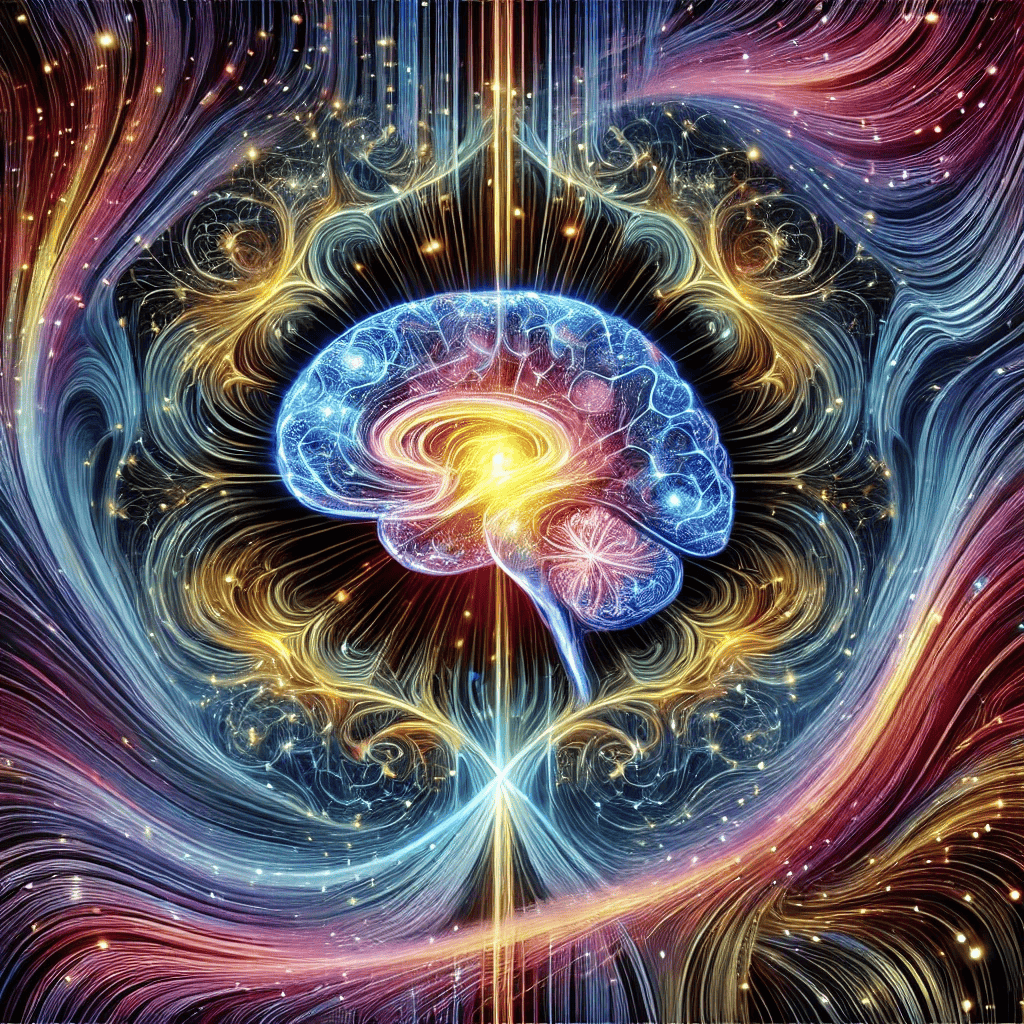
\includegraphics[width=0.8\textwidth]{cover.png}

    \caption{Cover art for Energetically Coherent Computation}
\end{figure}

\vspace{1cm}

\textit{This book was developed with significant reliance on advanced Large Language Models (LLMs), including Flux AI™, ChatGPT® and DALL·E® by OpenAI and Claude™ by Anthropic. These tools were instrumental in refining ideas, drafting and editing content, and even exploring and formulating mathematical models. While the core concepts and overarching framework remain my own, the collaborative nature of this work with LLMs has greatly shaped its structure and expression. Readers should understand this book as both an individual effort and a product of ongoing engagement with these transformative technologies.}

\vspace{2cm}

This work aims to establish a novel framework for understanding consciousness through an interdisciplinary synthesis spanning cognitive science, physics, and philosophy of mind. While computational approaches have proven remarkably successful in explaining many aspects of cognition, they face persistent challenges in accounting for phenomenal consciousness - the subjective, qualitative aspects of conscious experience.

The approach taken here attempts to bridge physical and computational perspectives. This theoretical framework, while speculative, draws on rigorous analysis of how phenomenology can link with current scientific understanding of the brain and engages with consciousness across cultural and historical contexts. A guiding intuition for this work is that the fundamental mysteries facing physics, biology, and psychology - the nature of energy, life, and consciousness respectively - may represent different aspects of a deeper theoretical challenge.

This work presents Energetically Coherent Computation (ECC) as a theoretical framework bridging multiple approaches to consciousness, but several important limitations warrant acknowledgment. While the framework offers mathematical sophistication, establishing clear empirical tests for its core claims remains a crucial challenge. The development of novel experimental methods to measure and manipulate patterns of energetic coherence will be essential for validating the theory's predictions.

The emphasis on energetic coherence should not be interpreted as dismissing the importance of neural computation. Rather than rejecting computational approaches, ECC suggests that computation alone cannot fully account for consciousness without considering its physical implementation through coherent energy dynamics. The framework aims to complement rather than replace computational understanding of neural processes.

The goal of this work is to suggest new ways of conceptualizing consciousness that bridge physical and experiential approaches while remaining open to refinement through future research. Readers are encouraged to approach these ideas critically while considering how they might be tested and developed through rigorous scientific investigation. Limitations notwithstanding, ECC offers valuable theoretical tools for understanding consciousness as simultaneously physical and experiential, suggesting productive directions for future research across multiple disciplines.

ECC aligns with Anil Seth's focus on addressing the "real" problem of consciousness - developing precise understanding of how phenomenology can be systematically influenced and controlled - rather than attempting to resolve the metaphysical challenges posed by the hard problem. As Phillip Goff argues, just as Maxwell advanced physics by assuming electromagnetic forces as fundamental while studying their behavior, consciousness research might progress by taking phenomenal experience as a basic feature of (of some part of) reality while investigating its organization and dynamics.

This pragmatic orientation acknowledges Thomas Nagel's fundamental insight about the apparent irreconcilability between first-person conscious experience and third-person scientific description. The "view from nowhere" that science attempts to achieve may be fundamentally incapable of capturing the subjective, qualitative aspects of consciousness. Rather than trying to bridge this explanatory gap, ECC focuses on understanding how physical patterns of energetic coherence relate to and influence conscious states while accepting the irreducibility of first-person experience.

By examining specific mechanisms through which patterns of energetic coherence shape conscious experience, ECC provides tools for addressing Seth's "real" problem - understanding consciousness well enough to enable precise control of phenomenal states. This creates opportunities for empirical investigation and potential therapeutic applications without requiring resolution of the deeper philosophical tensions Nagel identified between subjective and objective perspectives. The framework thus maintains scientific tractability while acknowledging the limitations of third-person approaches to understanding consciousness.

This approach suggests that progress in consciousness research may come not from trying to reduce phenomenal experience to physical description, but from developing increasingly sophisticated understanding of how physical processes and conscious experiences relate to and influence each other while remaining fundamentally distinct modes of reality. Just as physics advances without fully resolving questions about the ultimate nature of energy or matter, consciousness research can develop meaningful insights about the dynamics and control of experience while accepting certain philosophical limitations as fundamental rather than provisional.

As mentioned above, this work has been done with heavy use of modern large language models (LLMs) like Claude's Sonnet and ChatGPT's 4o. As of the 0.3.0 release, the references used in this document are still being revised for veracity (do they exist?) and fidelity (do they connect to the main text?). The text itself is also under revision - it presents a lot redundancy throughout and some contradictions between sections. Furthermore, not all sentences fully represent the views of the main author or may yet be misconstrued. A lot of (full time) work is still required to get this manuscript up to high academic standards. Thus, we advise the reader to engage with the text as a work in progress (a roadmap of sorts, more than a finished product) until a first edition is released. Pull requests and critiques are welcome on the \href{https://github.com/bobaseb/energetically-coherent-computation}{Github page}.